% --------------------------------------------------------------------------------
\newpage
\section{Roughness experiments}
% --------------------------------------------------------------------------------

% Make target for following functions:
\hypertarget{Concepts:IPEMRoughnessDemo}{}
\hypertarget{Concepts:IPEMGenerateANIForRoughnessTest}{}
\hypertarget{Concepts:IPEMGenerateANIForScales}{}
\hypertarget{Concepts:IPEMRoughnessRun}{}

\subsection{Introduction}
% --------------------------------------------------------------------------------
The \hyperlink{Concepts:Roughness Module}{Synchronization Index
Model}, which forms the kernel of the Roughness Module (RM), is
based on the idea that roughness depends on the degree in which
neurons synchronize with the beating frequencies. The model
provides a straightforward visualization of the components
contributing to roughness.

In this demonstration the Roughness Module is compared with
behavioral data in psychoacoustics and music psychology. Due due
the fact that a lot of sounds are processed, this demonstration
consumes time and hard disk memory. The output needs about
253MBytes of your hard disk. Performing the full demonstration
takes about 29 minutes on a Windows NT 4.0 system with Pentium
III 600 MHz processor, 256Mb RAM PC130.

% --------------------------------------------------------------------------------
\subsection{Method}
% --------------------------------------------------------------------------------

\IPEMTBC

%\subsubsection*{Framework}
%% --------------------------------------------------------------------------------
%The synchronization index model involves two concepts of
%band-pass filtering:
%\begin{itemize}
%\item
% A concept related to the resonance
%properties of the basilar membrane (=cochlear mechanical
%filtering).
% The width of the band-pass filters that simulate the
%resonance properties simulate the excitation on the basilar
%membrane. The equal width of excitation along the membrane
%corresponds to a quasi-logarithmic relationship in the frequency
%domain. We adopted the Auditory Peripheral Module from Van
%Immerseel and Martens \cite{VanImmerseel:92} but any model of the
%auditory periphery can be used in principle provided that it
%transforms sound into rate-code patterns at the level of the
%auditory nerve. The essential feature of the peripheral model is
%that it introduces the low frequencies in to the spectrum (owing
%to wave rectification).
%\item
%A type of band-pass filtering related to the synchronization of
%neurons to particular frequencies.\
% The upper limit of synchronization in the auditory nerve, which was implemented in
%the Auditory Peripheral Module at 1250 Hz, is clearly too high to
%account for sensory dissonance and roughness. Conceptually,
%synchronization can be divided into three regions corresponding
%to loudness (from 0 to about 25 Hz), to roughness and sensory
%dissonance (from 25 to about 300 HZ), and to pitch (roughly from
%300 to 1250 Hz). The synchronization model has a focus on the
%region between 25 to 300 Hz, which is known to be the frequency
%region of roughness.
%\end{itemize}
%
%The synchronization index model then calculates the roughness by
%a Fourier analysis of the beating frequency range and summing the
%normalized Fourier (magnitude-related) coefficients that
%represent the modulation depth of the beating frequencies. A
%global range for beating frequencies, however, cannot be
%maintained in all auditory channels. In particular, the
%synchronization filtering seems to rely on more narrow band-pass
%filters in the auditory channels whose central frequency is $<$
%800 Hz.


\subsection{Application}
% --------------------------------------------------------------------------------
\subsubsection*{Some Practical Considerations}
% --------------------------------------------------------------------------------
The contents and the functions of the demonstration package for
the roughness experiments can be found in the directory
IPEM$\backslash$Demos$\backslash$Roughness. To perform the
experiments execute the main script
\hyperlink{FuncRef:IPEMRoughnessDemo}{IPEMRoughnessDemo} for
demonstrating the calculation methods of roughness. The function
\hyperlink{FuncRef:IPEMGenerateANIForRoughnessDemo}{IPEMGenerateANIForRoughnessDemo}
generates all the files for the tests contained in the roughness
demo:
\begin{itemize}
\item
\hyperlink{FuncRef:IPEMGenerateANIForRoughnessTest}{IPEMGenerateANIForRoughnessTest}
(IPEMGenerateANIForRoughnessDemo Part I) generates sounds and
auditory nerve images for the psychoacoustical tests. The sounds
and images are further processed with IPEMRoughnessDemo (Part II).

\item
\hyperlink{FuncRef:IPEMGenerateANIForScales}{IPEMGenerateANIForScales}
(IPEMGenerataANIForRoughnessDemo Part II) generates an ANI and
soundfile of several harmonic and inharmonic sounds for the
musical tests.
\end{itemize}

The output, a number of mat-files containing the required auditory
nerve images and the soundfiles, is stored in the directory
RoughnessDemo relative to IPEMRootDir ('output').  The function
\hyperlink{FuncRef:IPEMRoughnessRun}{IPEMRoughnessRun} then calculates roughness of all the specified auditory nerve images using
different models and parameters.

\subsubsection*{Psychoacoustical tests}
% --------------------------------------------------------------------------------
This section compares the model's output with psychoacoustical
data. We start with amplitude modulated signals because they are
characterized by a few parameters whose effect of roughness has
been studied by many authors. We consider the effects of
modulation depth ($m$), amplitude ($A$), carrier frequency
($f_c$), and modulation frequency ($f_m$).

\begin{enumerate}
\item {\textbf{Modulation depth}}
    The dependency of the roughness $R$ on the degree of modulation
    $m$ has been expressed as a power law $R \sim m^n$. Depending on
    the experimental setup, $n$ can slightly vary from $1.2$ up to
    about $2$ \cite{Terhardt:97}. Figure (\IPEMTBC ask Marc)
    \ref{Fig:RoughnessExperimentsModulationDepth} shows the roughness of an amplitude
    modulated tone with $f_c$ 1000 Hz, $f_m$70 Hz, 60 dB in function
    of the modulation depth $m$ linearly increasing from 0 to 1.
    \begin{figure}[h]
        \centering
        
\includegraphics[width=\IPEMDefaultFigureWidth]{Graphics/MissingFigure}
        \caption{Calculated roughness as a function of modulation index $m$ =
        0...1 for a 1000 Hz AM tone}\label{Fig:RoughnessExperimentsModulationDepth}
    \end{figure}
    The dotted line shows the relation $R \sim m^{1.3}$ for $m \leq
    1$. The slope of this curve depends on the parameter $\delta$
    (see Equation \ref{normalizedRoughness}) which was set to 1.5 to obtain
    this result. A change of $\delta$ has a slight effect on the
    slope of the curve in Fig.~\ref{Fig:RoughnessExperimentsModulationDepth}.

\item {\textbf{Amplitude}}
    The effect of amplitude is illustrated in Fig.~\ref{Fig:RoughnessExperiments6}
    using an AM tone with $f_c$ 1000 Hz, $m = 1$, $f_m$ 50 Hz, and a
    linear decrease of SPL dB from 70 to 0. The dynamic range of
    neurons is known to be limited in the order of 30-50 dB. However,
    the large dynamic range of the human auditory system is explained
    by the spread of excitation due to the resonance characteristics
    of the basilar membrane \cite{Smith:88}. The spread of excitation
    is reflected in figure ~\ref{Fig:RoughnessExperiments26}a where a broad excitation
    range can be noticed at a level of 70 dB. This range narrows down
    as the level decreases. In figure ~\ref{Fig:RoughnessExperiments26}b, however, one
    may notice that the excitations contribute to the same frequency
    of 50 Hz. From 70 to about 53 dB the roughness halves.
    \begin{figure}[h]
        \centering
        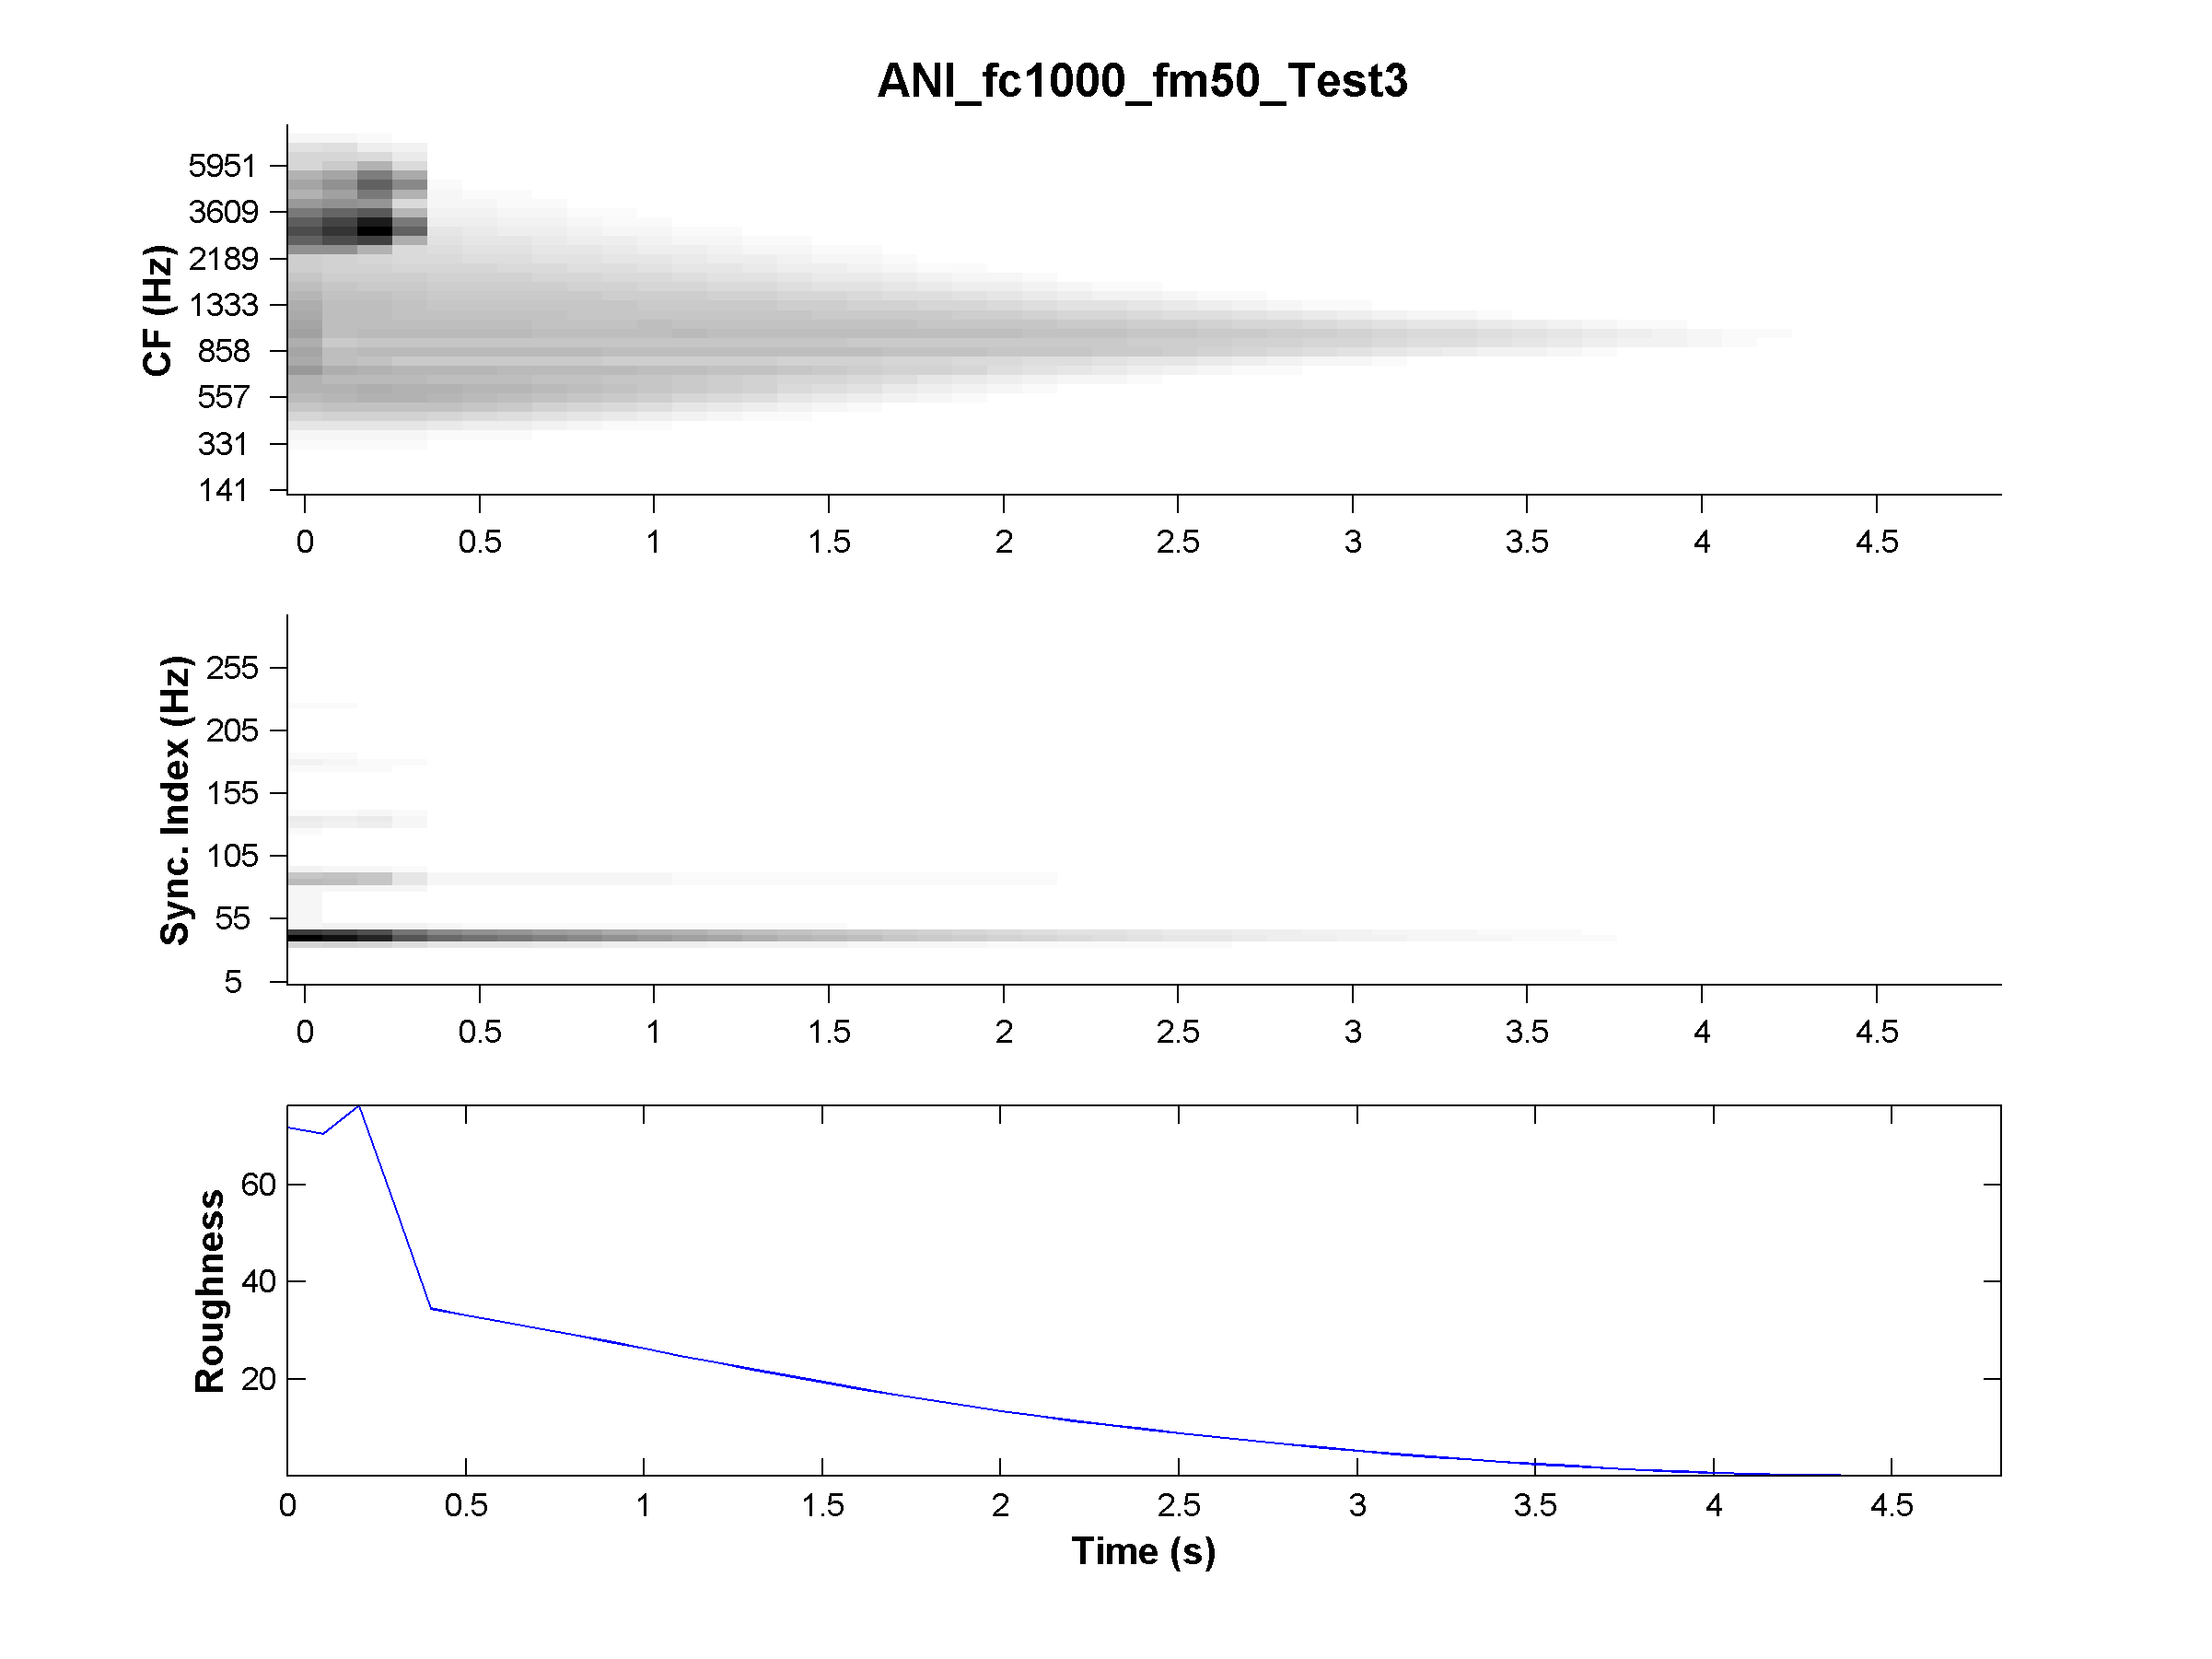
\includegraphics[width=\IPEMDefaultFigureWidth]{Graphics/RoughnessExperiments26}
        \caption{Calculated roughness as a function of amplitude.}
        \label{Fig:RoughnessExperiments26}
    \end{figure}

\item {\textbf{Frequency Modulation}}
    The formula used to calculate an FM tone is
    \cite{DanielWeber:1997}:
    \begin{displaymath}
        s(t) ~=~ \hat{s}.
        sin \left( 2 \pi f_c t - \frac{\Delta f}{f_{mod}}. cos (2 \pi f_{mod} t) \right)
    \end{displaymath}
    where $\hat{s}$ is the effective amplitude. The effects of
    frequency modulation on roughness show a band-pass characteristic
    with maximal values from 40 Hz to 70 Hz \cite{Kemp:1982}
    figure~\ref{Fig:RoughnessExperimentsKemp1}, full line), which our model (dotted line)
    approximates except at $f_{mod}$ 20 Hz, where the estimated
    roughness is clearly too high. The other values fall within the
    quartile range. The signal is
    a 1.6 kHz FM tone at 60 dB with $\Delta f$ 800 Hz whose  roughness
    is measured at $f_{mod}$ 1 10 20 40 60 80 100 200 300 400 500
    Hz.

    \begin{figure}[p]
        \centering
        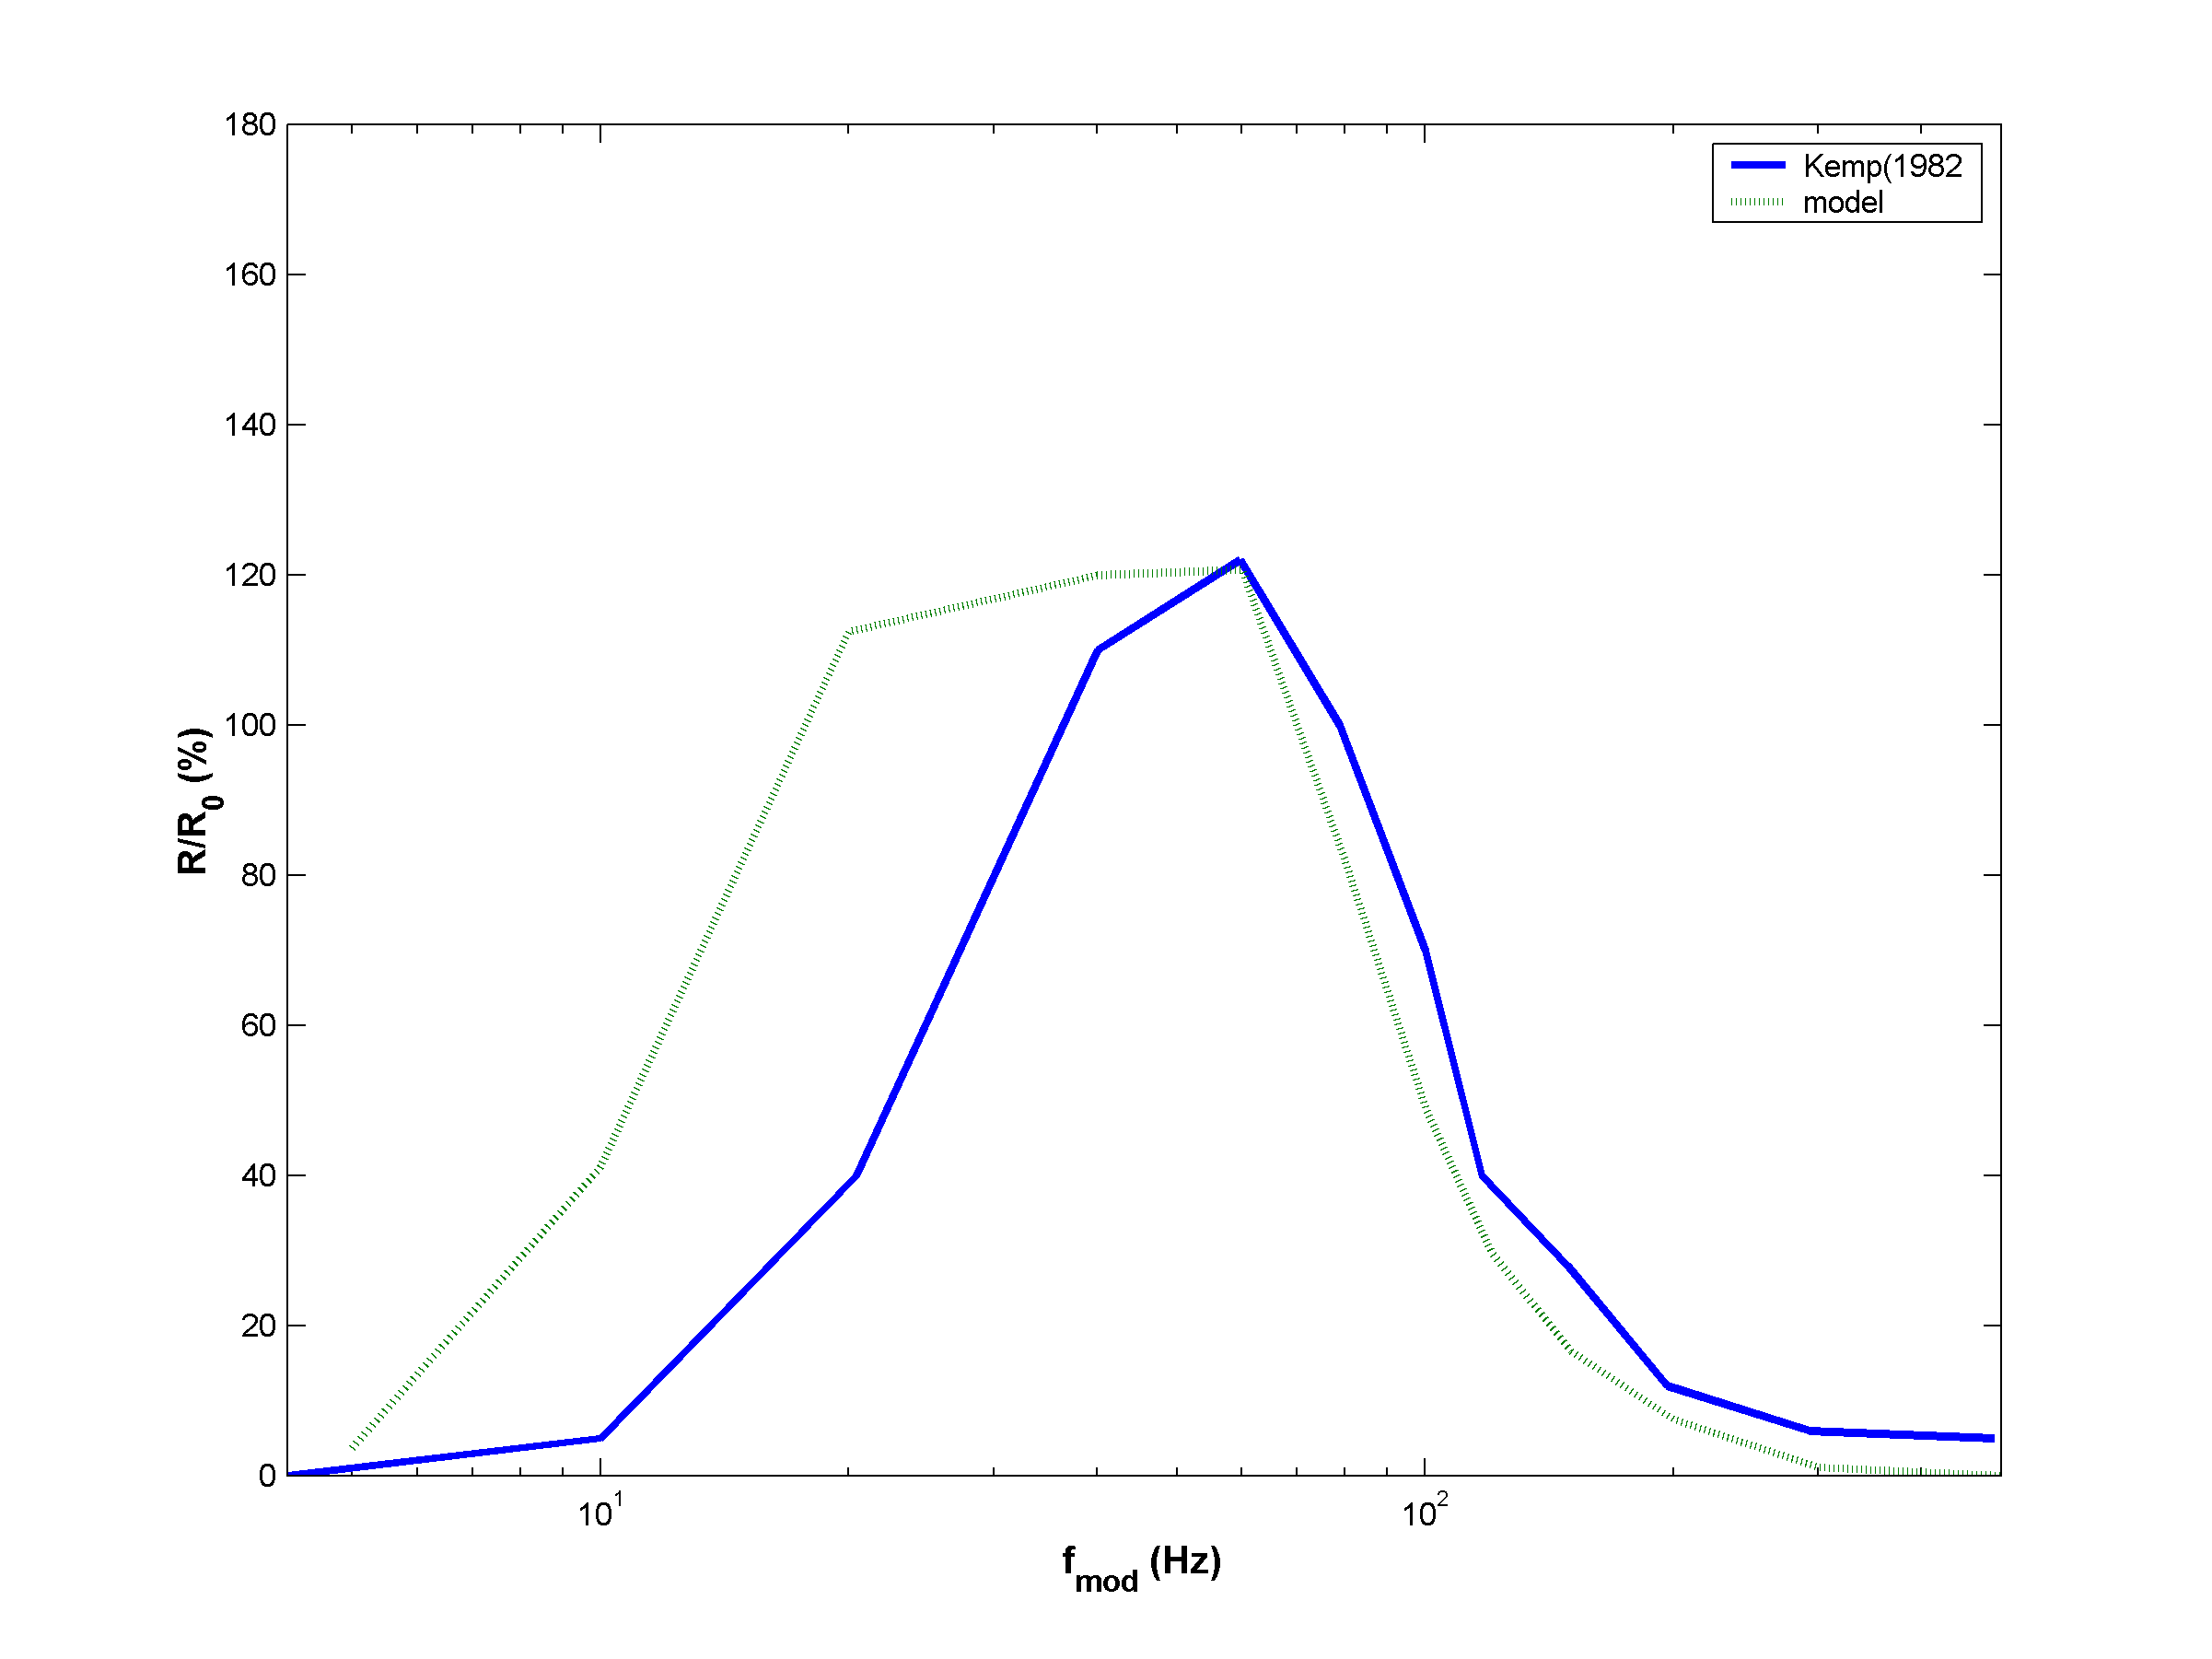
\includegraphics[width=\IPEMDefaultFigureWidth]{Graphics/RoughnessExperimentsKemp1}
        \caption{Calculated roughness as a function of frequency modulation. The signal is
        a 1.6 kHz FM tone at 60 dB with $\Delta f$ = 800 Hz, and $f_{mod}$
        from 1 10 20 40 60 80 100 200 300 400 500 Hz. The peaks are
        generated at the onsets}
        \label{Fig:RoughnessExperimentsKemp1}
    \end{figure}

    In addition, the roughness of a FM tone with $f_c$ 1600 Hz,
    $f_{mod}$ 70 Hz, at 60 dB is measured in function of the frequency
    deviation $\Delta f$ at 10 15 30 60 120 160 340 580 880 1130 1400
    1580 1720 Hz (figure ~\ref{Fig:RoughnessExperimentsKemp2}). The results correspond
    rather well with the available psychoacoustical data, as shown in
    figure ~\ref{Fig:RoughnessExperimentsKemp1}. (All values fall within the quartile
    range).
    \begin{figure}[p]
        \centering
        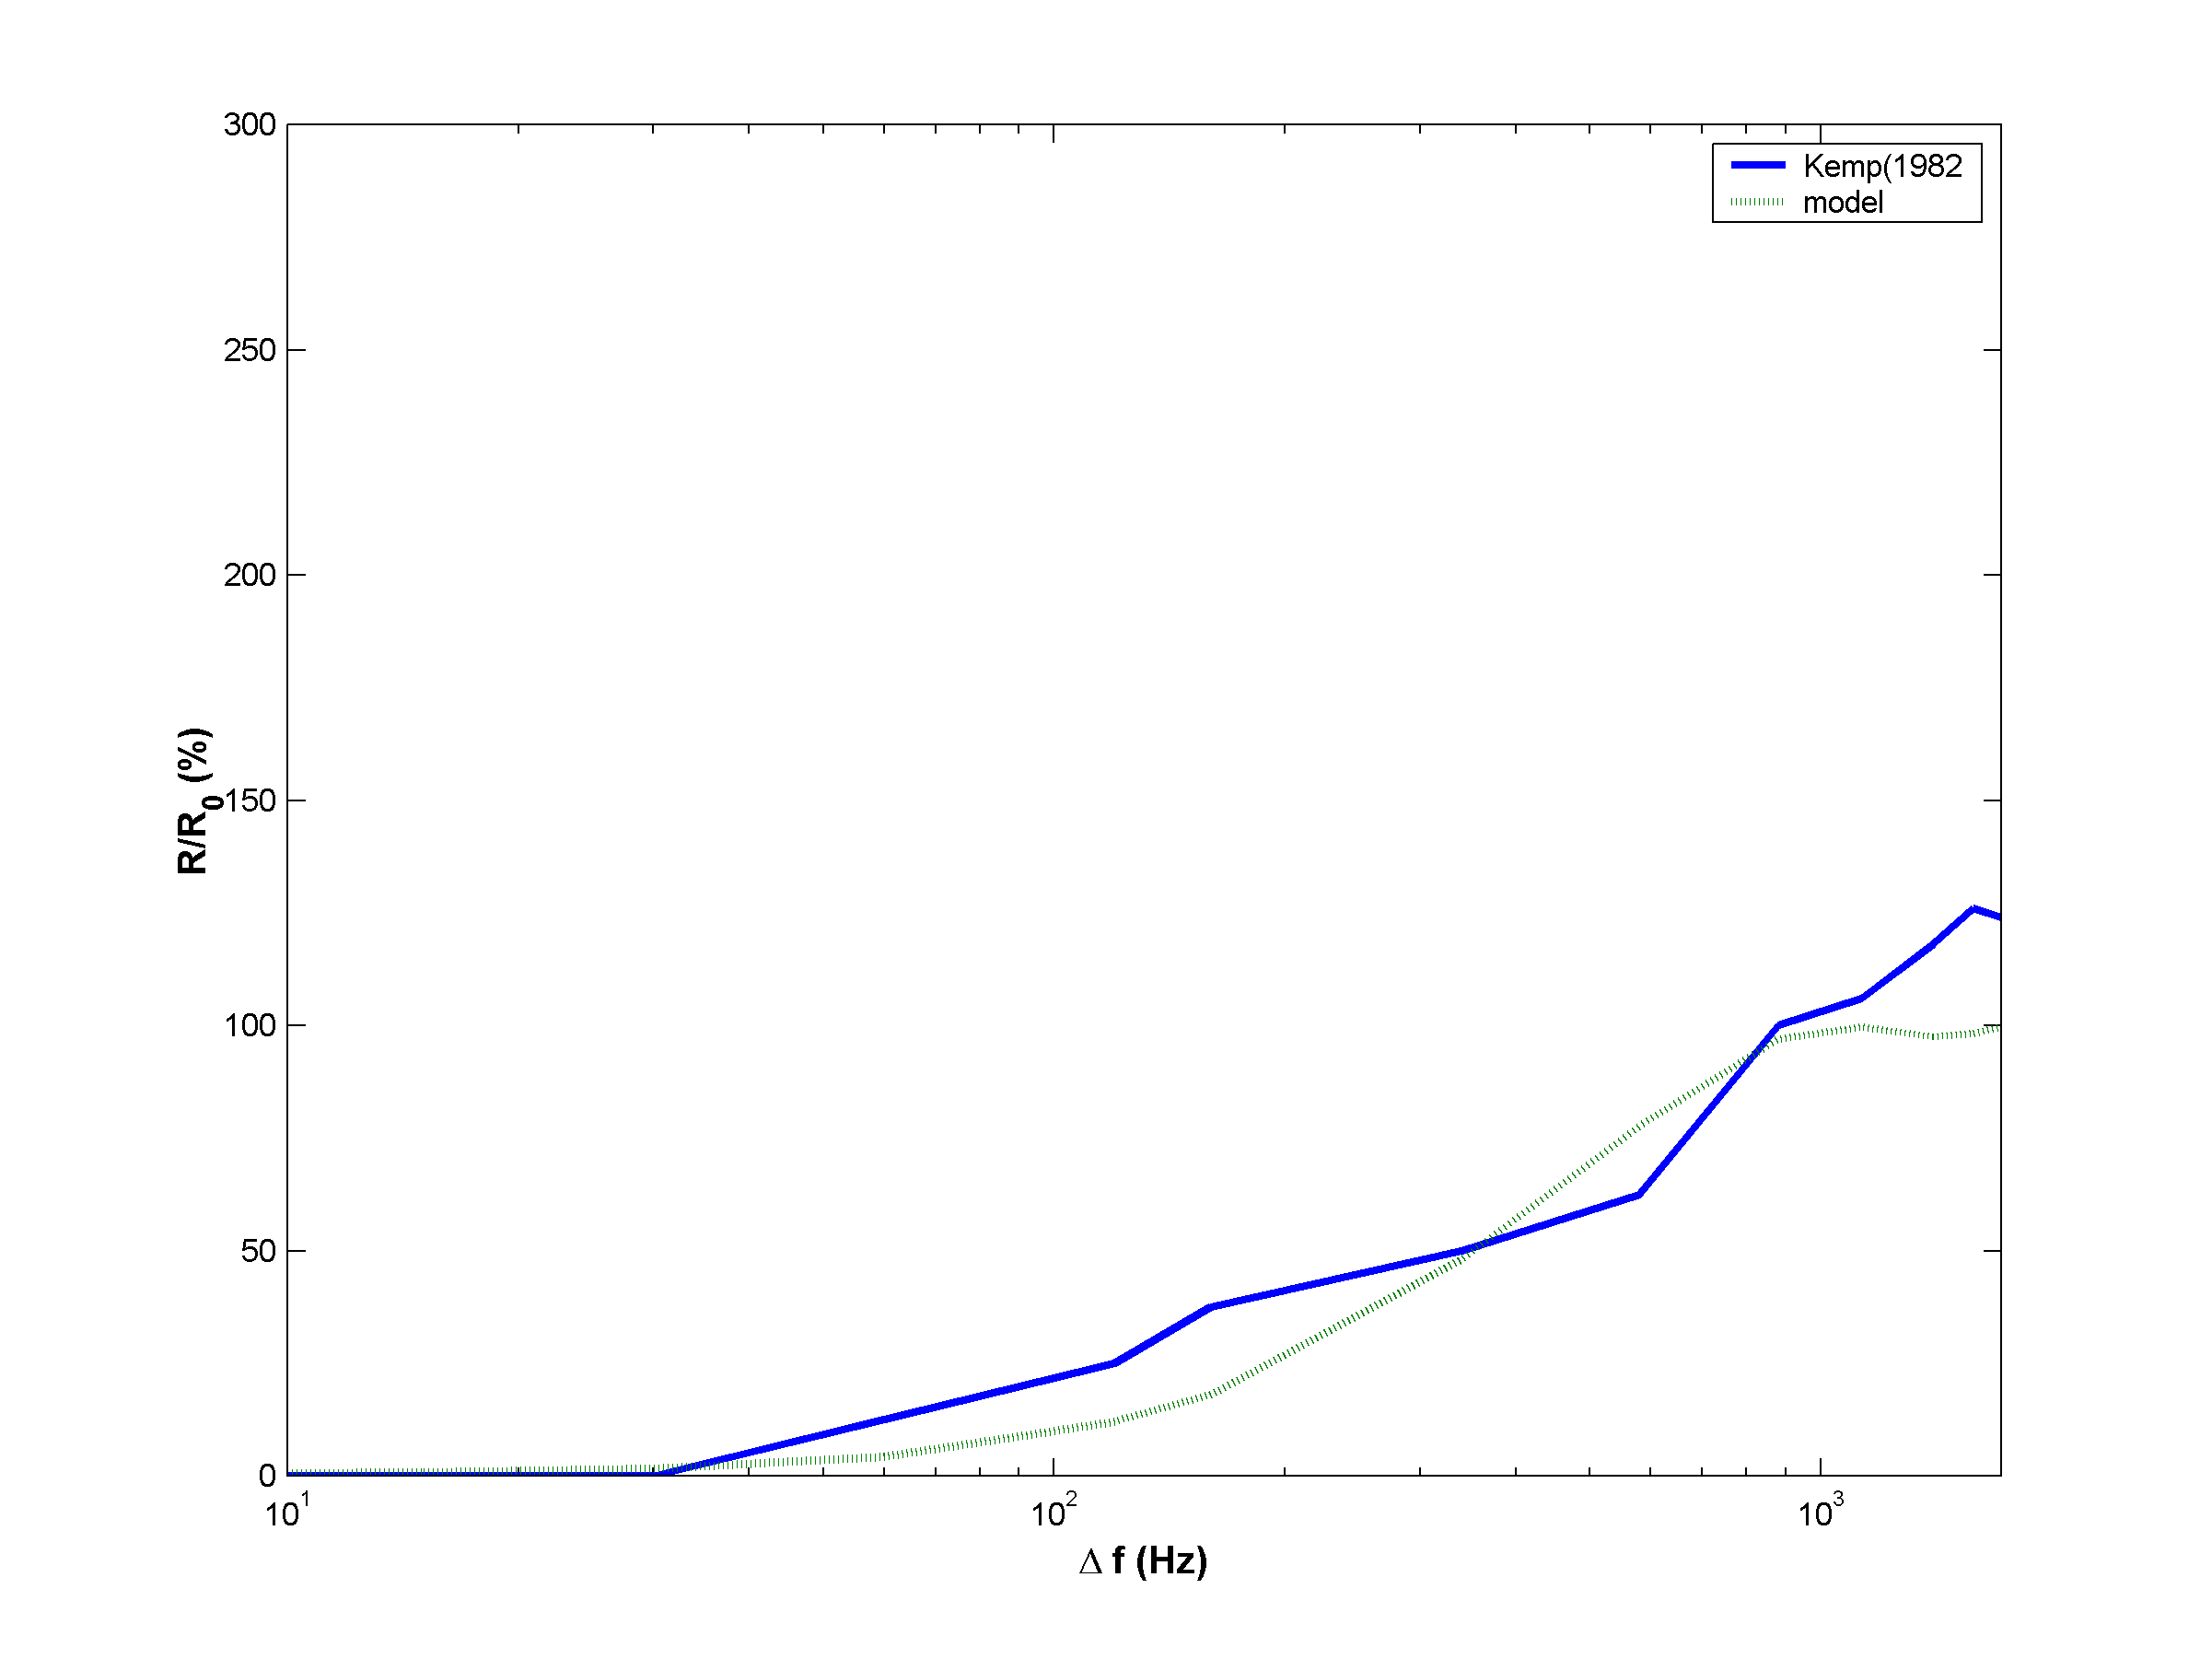
\includegraphics[width=\IPEMDefaultFigureWidth]{Graphics/RoughnessExperimentsKemp2}
        \caption{Comparison of the model's output (dotted line) with
        psychoacoustical data (full line). The signal is
        a 1.6 kHz FM tone at 60 dB with $\Delta f$ 800 Hz measured
        at $f_{mod}$ from 1 10 20 40 60 80 100 200 300 400 500
        Hz.}
        \label{Fig:RoughnessExperimentsKemp2}
    \end{figure}

\end{enumerate}

\subsubsection*{Musical tests}
% --------------------------------------------------------------------------------
The music theoretical interest of the concept of roughness is
demonstrated by taking a harmonic tone complex and playing it
together with a pitch shifted version thus specifying different
musical intervals of the timbre over a defined range. As an
illustration, we took a harmonic tone complex consisting of a
fundamental ($f_0$) at 500 Hz and 5 harmonics with equal
amplitude. This tone is played together with a pitch shifted copy.
The shift over 5 seconds is linear in frequency up to the upper
octave ($f_0$ 1000 Hz). The roughness as calculated with the
synchronization index model is shown in figure
~\ref{Fig:RoughnessExperiments31}.
\begin{figure}[p]
  \centering
  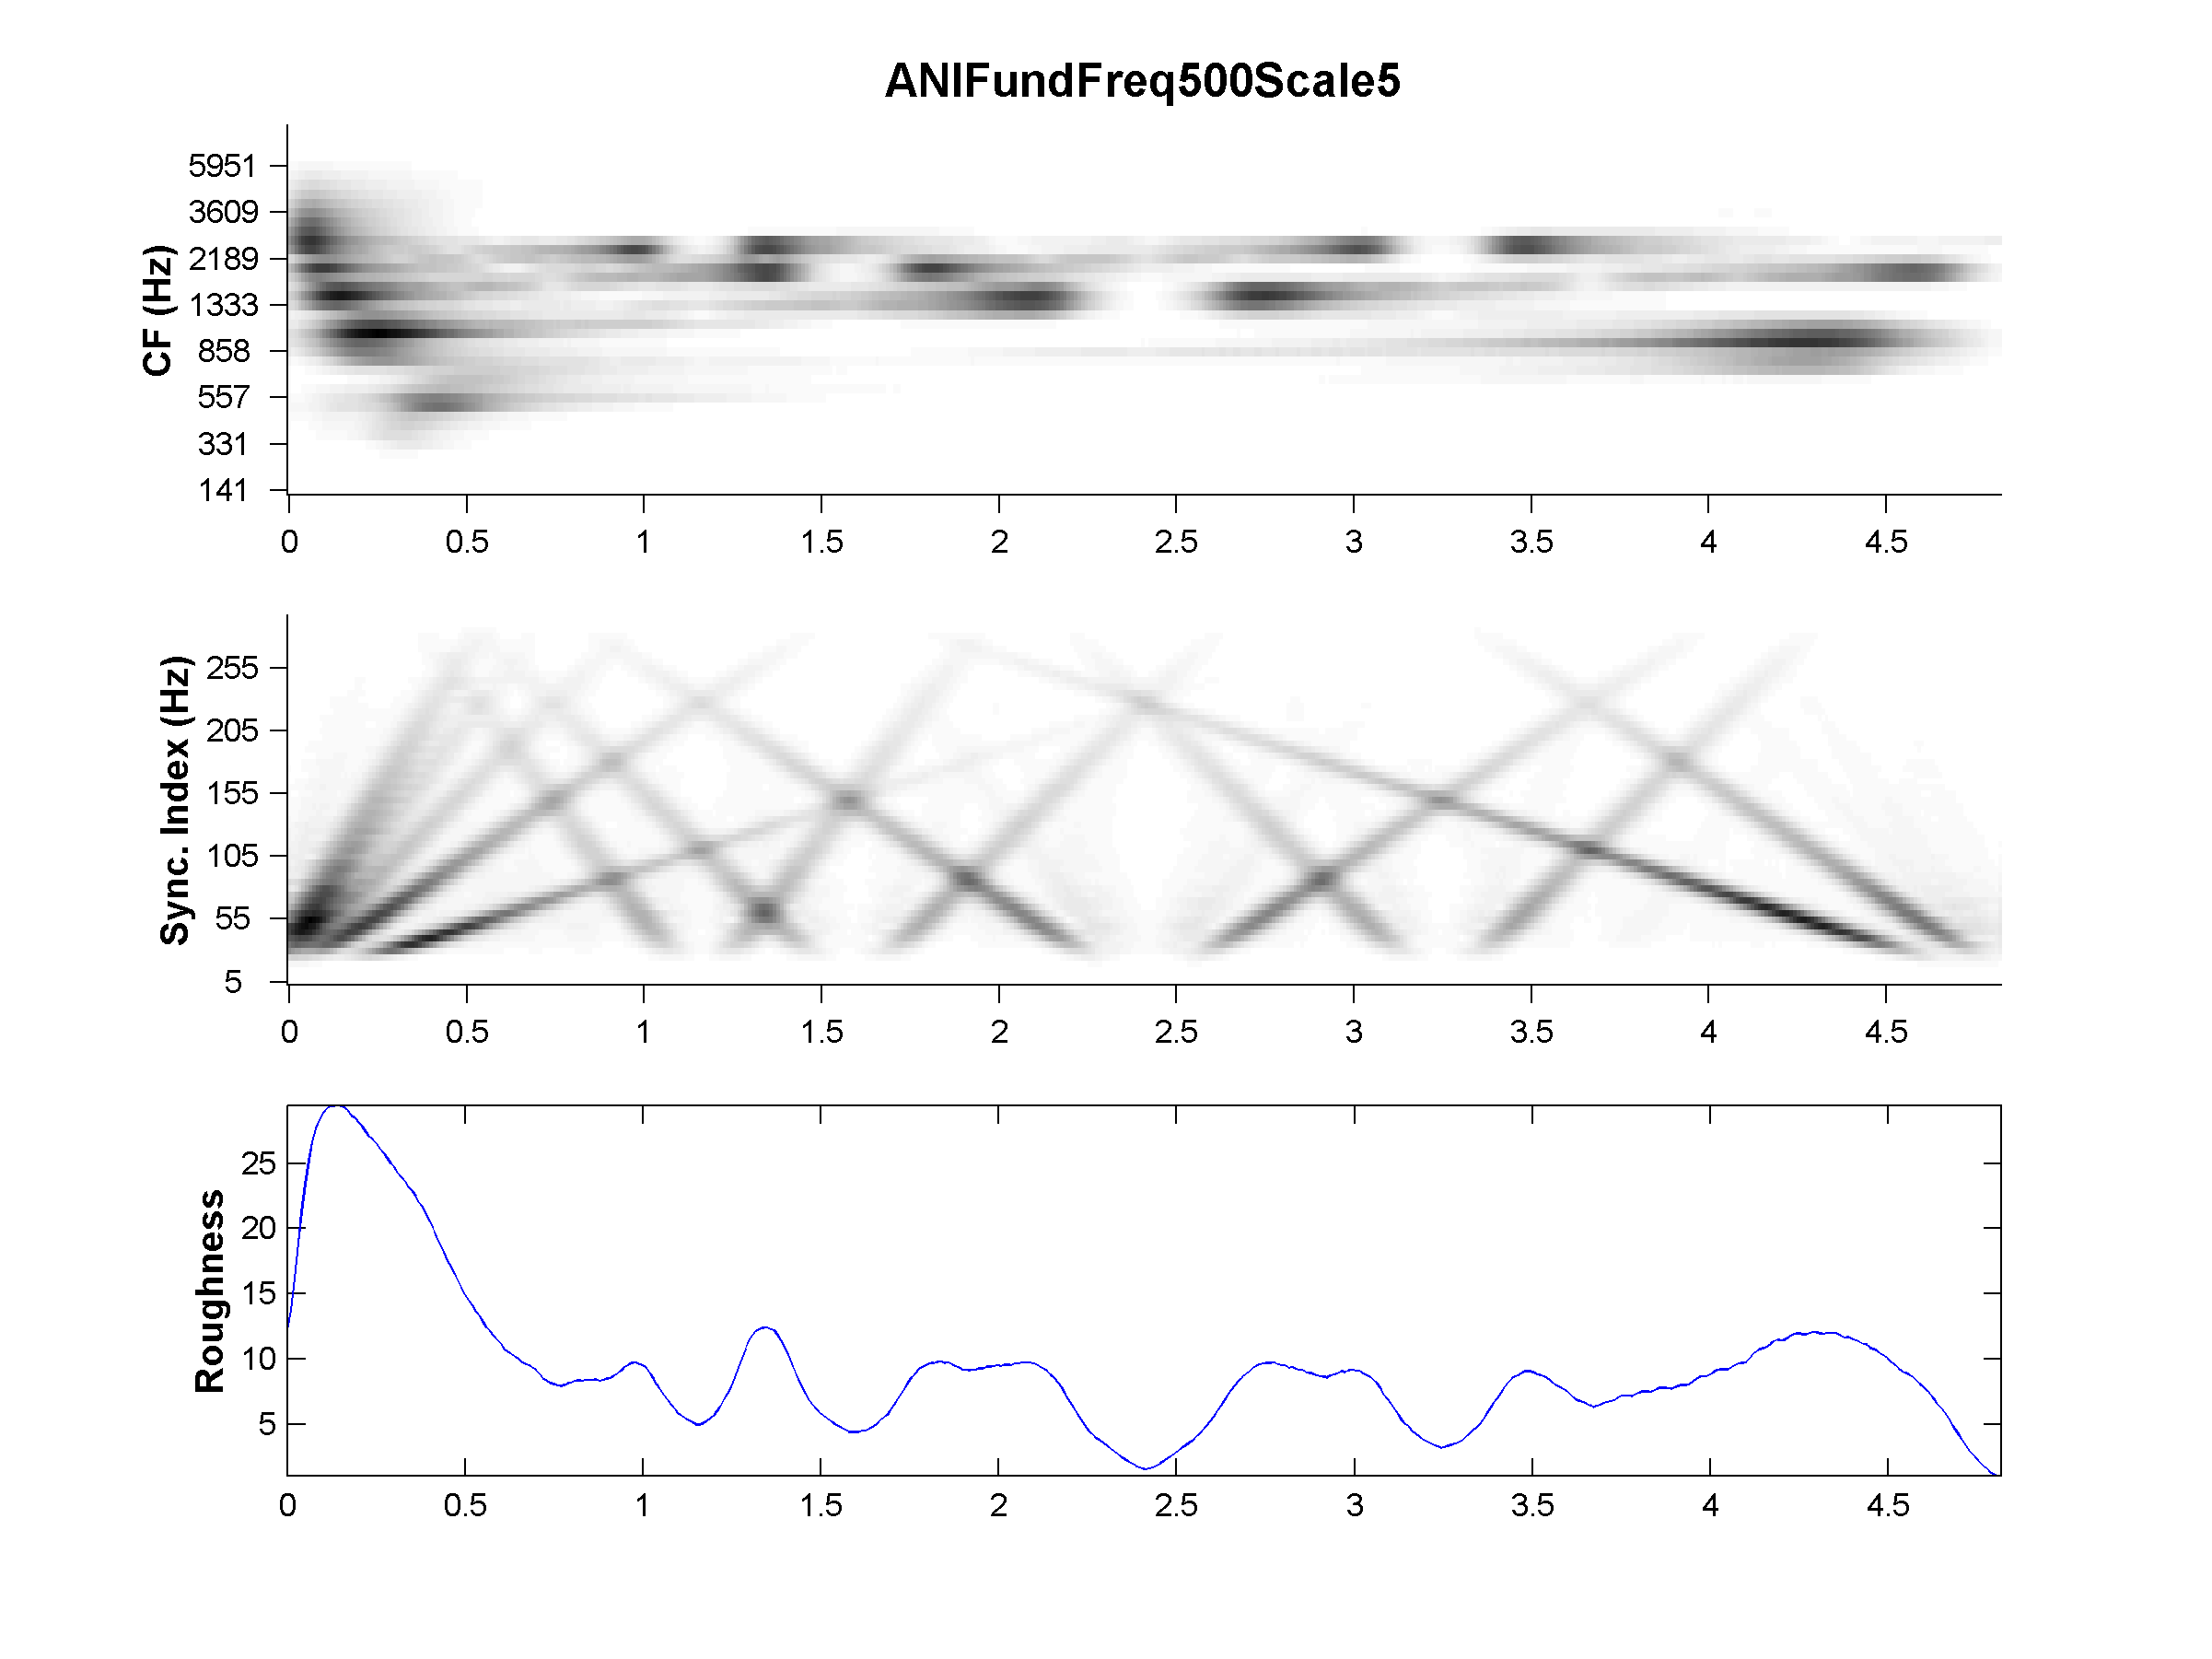
\includegraphics[width=\IPEMDefaultFigureWidth]{Graphics/RoughnessExperiments31}
  \caption{A harmonic tone complex with $f_0$ 500 Hz is played together with a
  pitch shifted copy (up to $f_0$ 1000 Hz). The harmonics have equal amplitudes.
  Top panel: excitation in the auditory channels.  Middle panel: synchronization
  index.
  Lower panel: roughness as calculated with the synchronization index model.}
  \label{Fig:RoughnessExperiments31}
\end{figure}

The roughness curve in figure ~\ref{Fig:RoughnessExperiments31}
can be compared with the results of the curve-mapping model of
roughness of \citeA{Sethares:98}(figure
~\ref{Fig:RoughnessExperiments30}). This model takes the
frequency-amplitude values as input (no sound!) and calculates the
curve using the psychoacoustical curve of \citeA{Plomp}. The
Synchronization Index Model (figure
~\ref{Fig:RoughnessExperiments33}), apart from its good agreement
with this theoretical model, provides an additional cue in showing
the 'spectral' (=excitation in the auditory channels) as well as
'temporal' (=synchronization index profile) factors that
contribute to roughness. Note that the dips are less deep than in
Sethares' model, which is partly due to the fact that the model
works on a glissando of harmonic tone complexes, rather than on
separate intervals. The points of minimal roughness indicate a
hierarchical order of intervals in terms of roughness. This
hierarchy can be musically exploited as the points of minimum
roughness may indicate candidates for a musical scale.

\begin{figure}
    \centering
    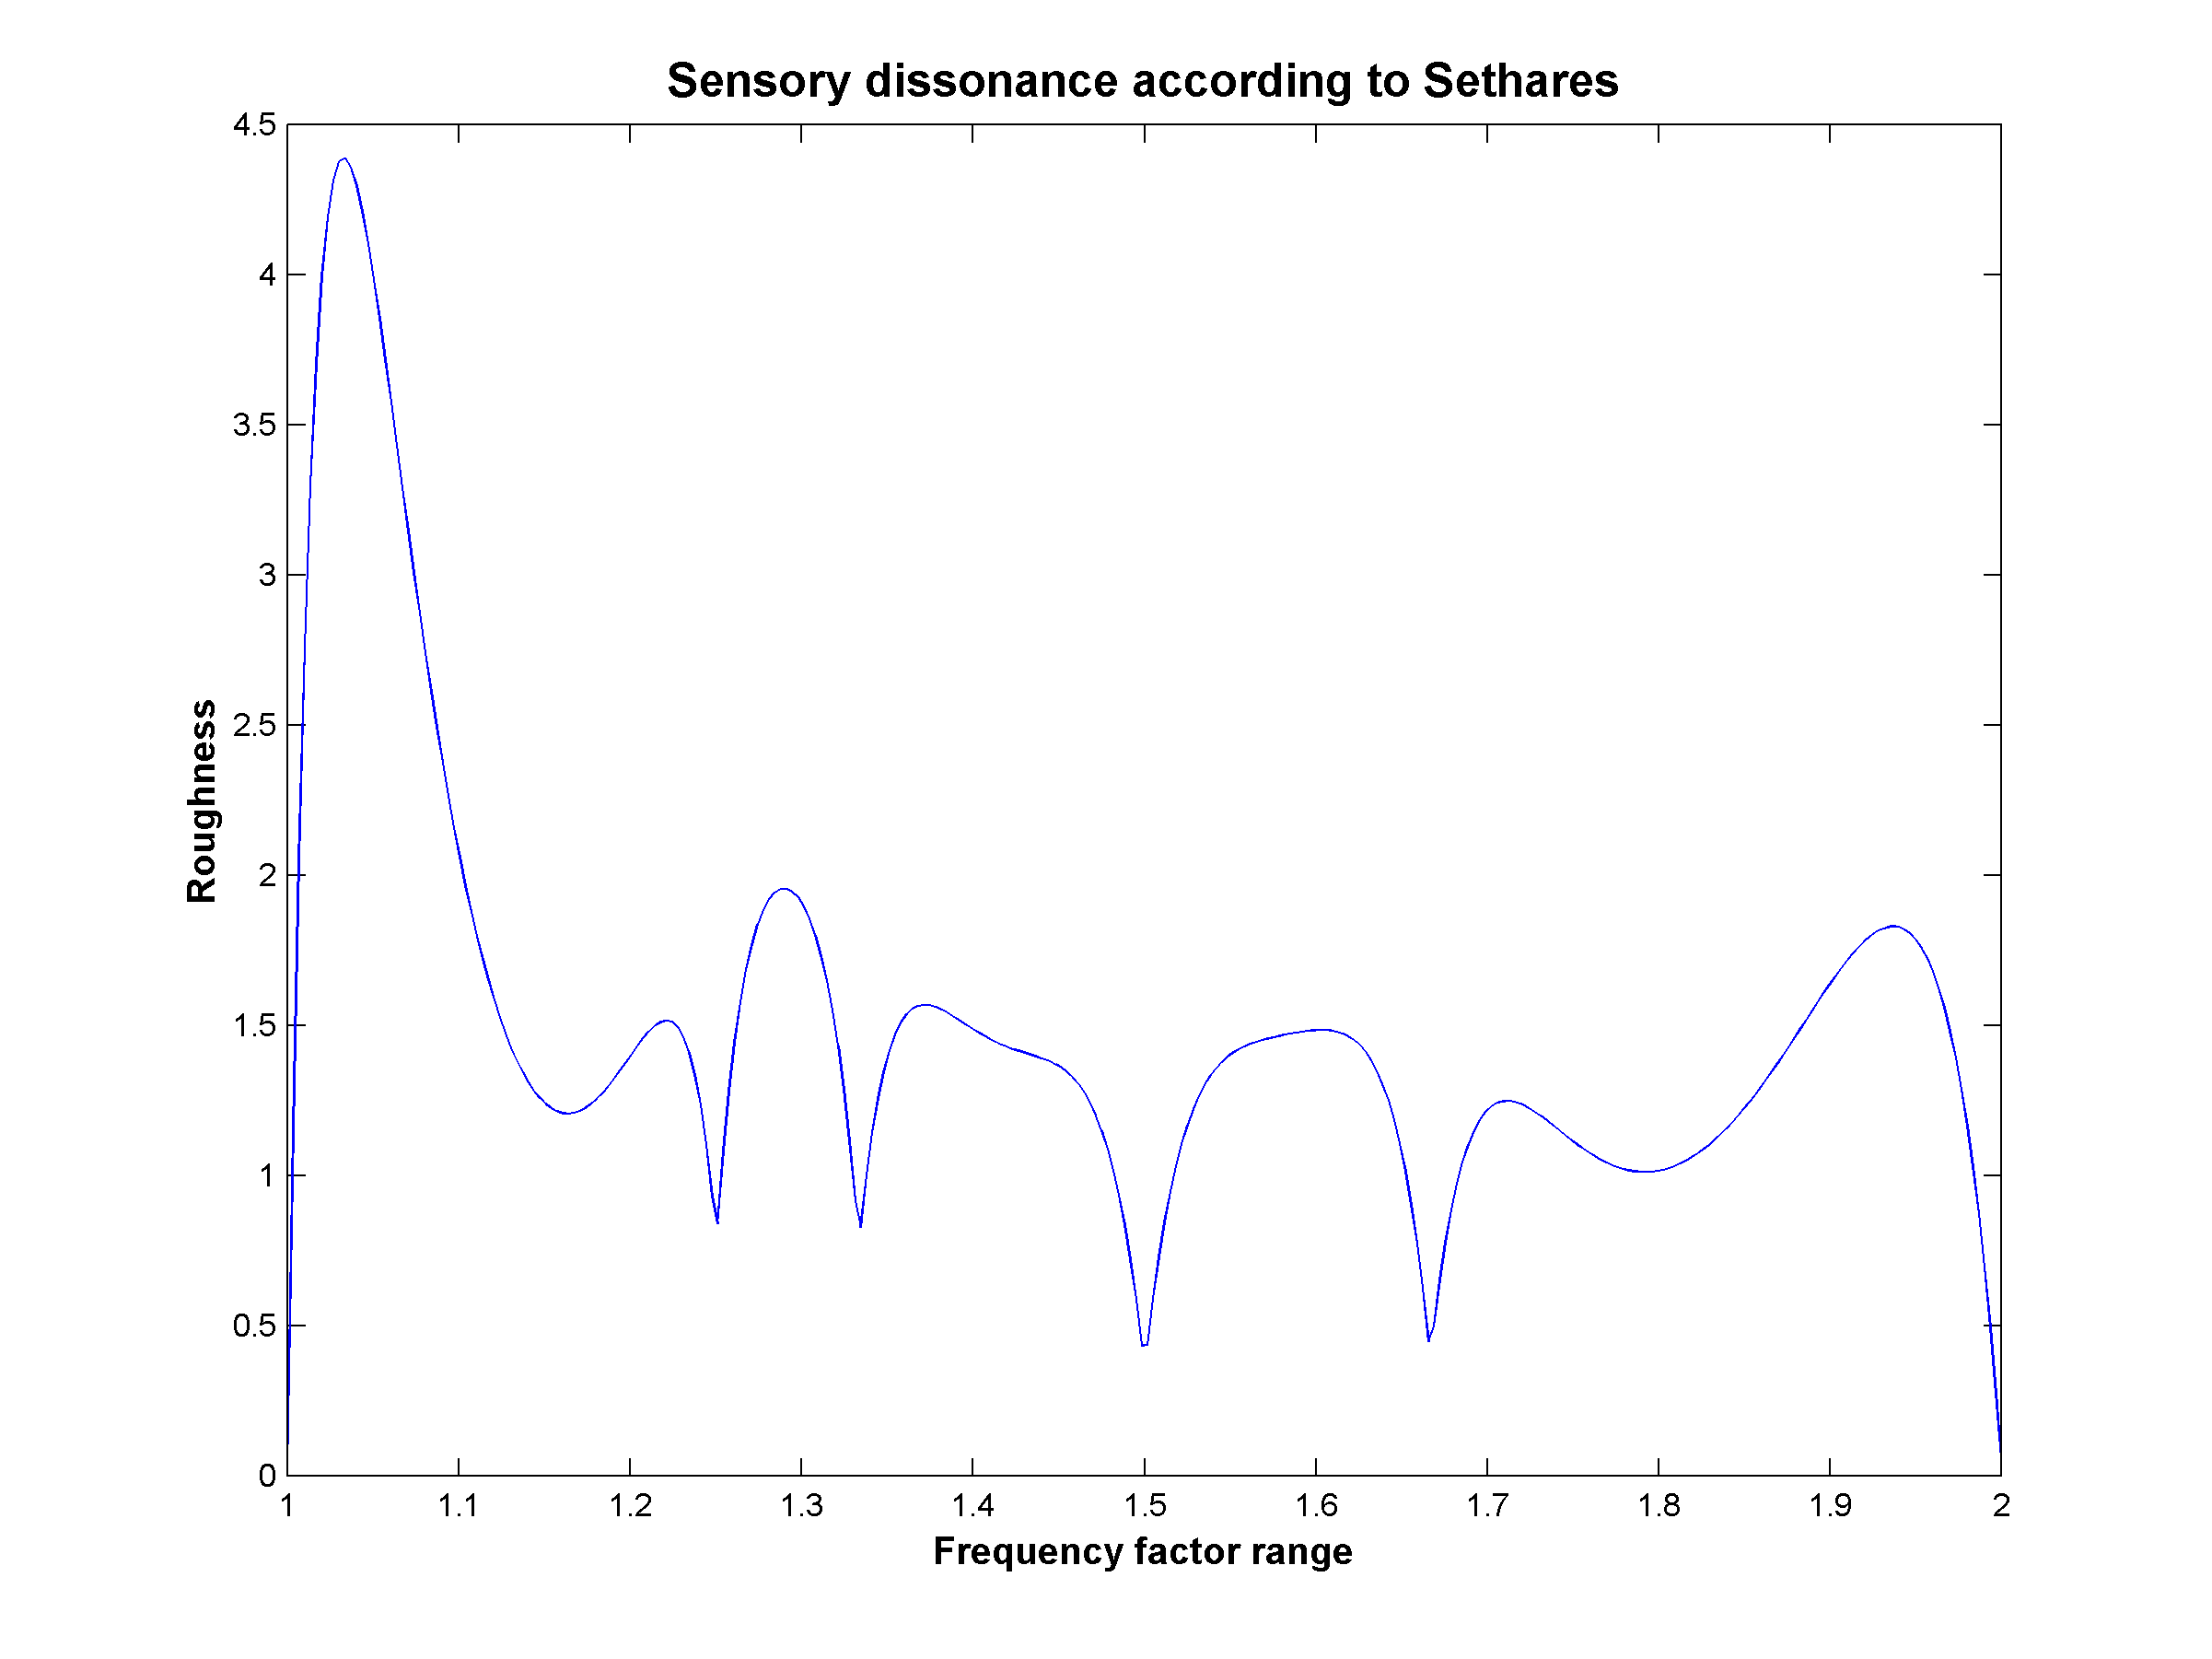
\includegraphics[width=\IPEMDefaultFigureWidth]{Graphics/RoughnessExperiments30}
    \caption{Sensory
    dissonance as calculated with the curve-mapping model of Sethares}
    \label{Fig:RoughnessExperiments30}
\end{figure}

\begin{figure}
    \centering
    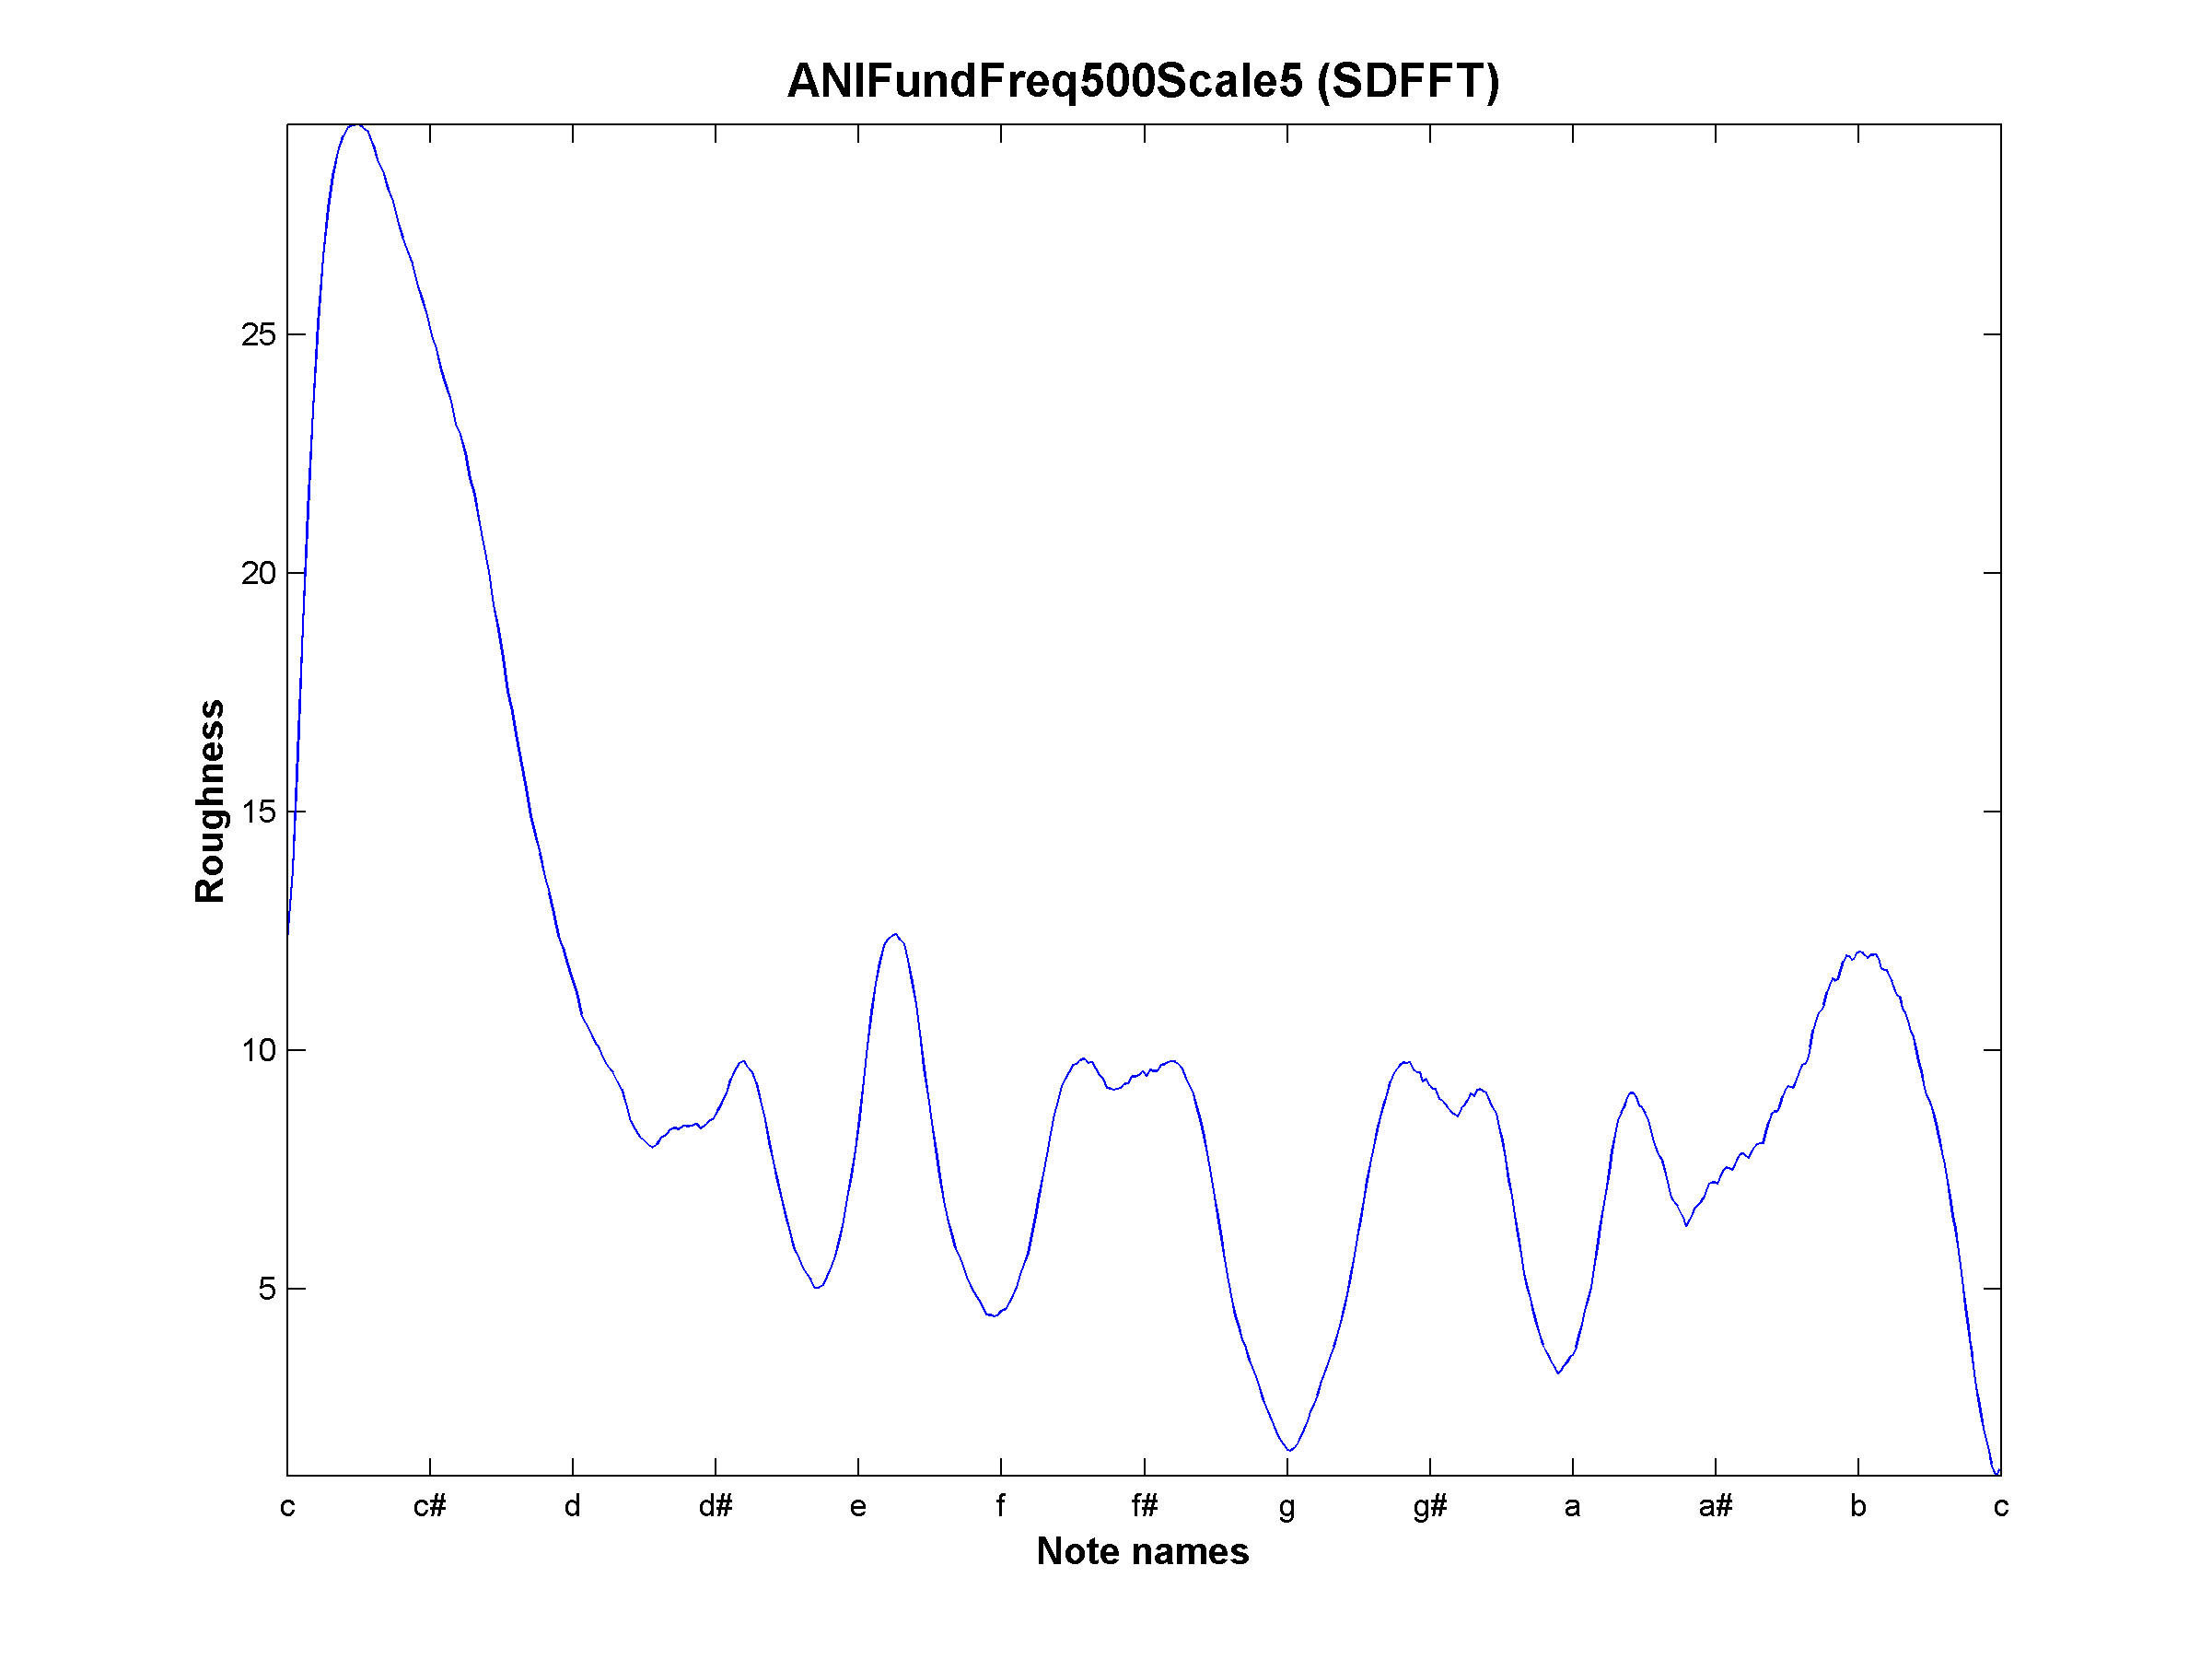
\includegraphics[width=\IPEMDefaultFigureWidth]{Graphics/RoughnessExperiments33}
    \caption{Roughness as calculated with the Synchronization Index Model}
    \label{Fig:RoughnessExperiments33}
\end{figure}

\subsection{Results and discussion}
% --------------------------------------------------------------------------------
\subsubsection*{Dependency}
% --------------------------------------------------------------------------------
The dependency of roughness on $m$, $f_m$ and $f_c$ provides
evidence for the theory that roughness may be directly related to
the degree in which neurons synchronize with the beating
frequencies of the AM tones. Roughness should then depend on two
basic effects:
\begin{itemize}
\item
The 'spectral' filtering resulting from the resonance properties
of the basilar membrane.
\item
The neuronal synchronization and its possible limitations.
\end{itemize}

\subsubsection*{Modulation frequency smaller than 25 Hz}
% --------------------------------------------------------------------------------
For $f_m$ smaller than about 25 Hz, the sensation of roughness
goes over into a sensation of fluctuation and loudness. Roughness
starts at about $f_m > 25 $ Hz but then the effects of spectral
filtering and synchronization should be taken into consideration.

\subsubsection*{Frequencies outside the filter bandwith}
% --------------------------------------------------------------------------------
AM tones have spectral energy at both sides ($f_c \pm f_m$) of a
carrier frequency $f_c$. An increase of the modulation frequency
$f_m$ results in a widening of the intervals. Consequently, when
the side frequencies ($f_c \pm f_m$) fall outside the central
scope of the $f_c$ filter bandwidth, their energy becomes more
and more attenuated and the beating decreases in relation to
that. The bandwidth of the auditory filters corresponds to
resonance regions of equal distance on the basilar membrane
\cite{GreenwoodJoris:1996}. Due to the quasi logarithmic
relationship between distance and frequency, the filter bandwidth
of this filter becomes broader in the higher frequency regions.
The 'spectral' filtering that results from the resonance
properties of the basilar membrane accounts for the fact that the
roughness decreases when $f_m$ exceeds the bandwidth of the
filtering associated with $f_c$. As the frequency components
exceed the bandwidth of an auditory filter, they will no longer
interfere and will cease to produce beating frequencies.

\subsubsection*{Frequency components within the filter bandwidth}
% --------------------------------------------------------------------------------
In the case, when the frequency components fall within the
bandwidth of the spectral filter, the neurons will attempt to
synchronize to the beating frequencies provided that those
frequencies are not too fast. Analysis of neuronal responses in
the auditory nerve indicates that neuronal synchronization has an
upper limit at about 1000 Hz which implies an absolute limit for
inferences based on synchronization \cite{JorisYin:1992}. But fast
beating frequencies, however, will be picked up as pitches rather
than roughness \cite{SchreinerLangnerNeuro:88a}. Only the beating
frequencies (e.g.~$25 Hz < f_m < 300$ Hz), will contribute to
roughness, suggesting that synchronization is actually subjected
to a band-pass filtering.

\subsubsection*{Conclusion}
% --------------------------------------------------------------------------------
The synchronization index model offers a standard method in the
calculation of the modulation depth for roughness. The method
allows a proper visualization of the features that contribute to
roughness both in terms of fluctuations in the auditory channels,
and in terms of phase-locking synchrony. The visualization
provides interesting cues for analyzing the factors that
contribute to roughness.
